\documentclass{beamer}
\usepackage{tikz}
\usepackage{booktabs}
\usetheme{Copenhagen}
\usecolortheme{default}
% Show page number on each frame
% Footline: Author (left) • Title (center) • Frame x / N (right)
\setbeamertemplate{footline}{
  \leavevmode
  \hbox{%
    \begin{beamercolorbox}[wd=.33\paperwidth,ht=2.5ex,dp=1ex,left]{author in head/foot}
      \usebeamerfont{author in head/foot}\hspace{1ex}\insertshortauthor
    \end{beamercolorbox}%
    \begin{beamercolorbox}[wd=.57\paperwidth,ht=2.5ex,dp=1ex,center]{title in head/foot}
      \usebeamerfont{title in head/foot}\insertshorttitle
    \end{beamercolorbox}%
    \begin{beamercolorbox}[wd=.10\paperwidth,ht=2.5ex,dp=1ex,right]{date in head/foot}
      \usebeamerfont{date in head/foot}\insertframenumber{} / \inserttotalframenumber\hspace{1ex}
    \end{beamercolorbox}%
  }
  \vskip0pt
}
\title[Phase 2 - Acoustic Signal Classification] %optional
{Automatic Scaling Bar}
\subtitle{Phase 2 - Acoustic Signal Classification}
\author[Kanwar Pannu] % (optional)
{Kanwar Pannu\\
Supervisors: Dr. Travis Wiens\inst{1}, Dr. Abdul Bais\inst{2}}

\institute[VFU]{%
  \textbf{Supervisors:} Dr.\ Travis Wiens\inst{1}, Dr.\ Abdul Bais\inst{2}\\
    \and
  \inst{1}College Of Engineering\\
  University of Saskatchewan
  \and
  \inst{2}Faculty of Engineering and Applied Science\\
   University of Regina
}

\date[] % (optional)
{}

% Use a simple TikZ graphic to show where the logo is positioned
\logo{\begin{tikzpicture}
\node[inner sep=0pt] (usask) at (0,0)
{
\includegraphics[width=20mm]{../assets/usask.png}};
\node[inner sep=0pt] (uregina) at (-2,0)
{
\includegraphics[width=15mm]{../assets/uregina.png}};
\node[inner sep=0pt] (nserc) at (-5,0)
{
\includegraphics[width=40mm]{../assets/NSERC_FIP_RGB.png}};
\node[inner sep=0pt] (giems) at (-8,0)
{
\includegraphics[width=10mm]{../assets/GIEMS_logo_colored.jpg}};
\node[inner sep=0pt] (imii) at (-10,0)
{
\includegraphics[width=20mm]{../assets/imii.png}};
\end{tikzpicture}
}

%End of title page configuration block
%------------------------------------------------------------
%The next block of commands puts the table of contents at the 
%beginning of each section and highlights the current section:

%------------------------------------------------------------
\begin{document}
{%
% hide page number on title
  \setbeamertemplate{author}{Kanwar Pannu}
  \frame{\titlepage}
}
\author{Kanwar Pannu}
\logo{} % <- clear logos after title page
%---------------------------------------------------------
%Highlighting text
\begin{frame}

\frametitle{What is a Scaling Bar?}

\begin{columns}[T,onlytextwidth]
  \begin{column}{0.68\textwidth}
    \begin{itemize}
      \item One common method of evaluating the safety of a roof is by using scaling bar impacts.
      \item Before entering a newly mined area or before starting work in an area, the worker will use a scaling bar (a steel or aluminum bar usually 2–3 m in length) to strike the roof in various locations.
      \item By listening to the sound of the impact, the worker can estimate whether that area of roof is likely to fall i.e.\ decide whether the sound is ``Drummy'' or ``Tight''.
    \end{itemize}
  \end{column}
  \begin{column}{0.32\textwidth}
    \begin{figure}
      \centering
      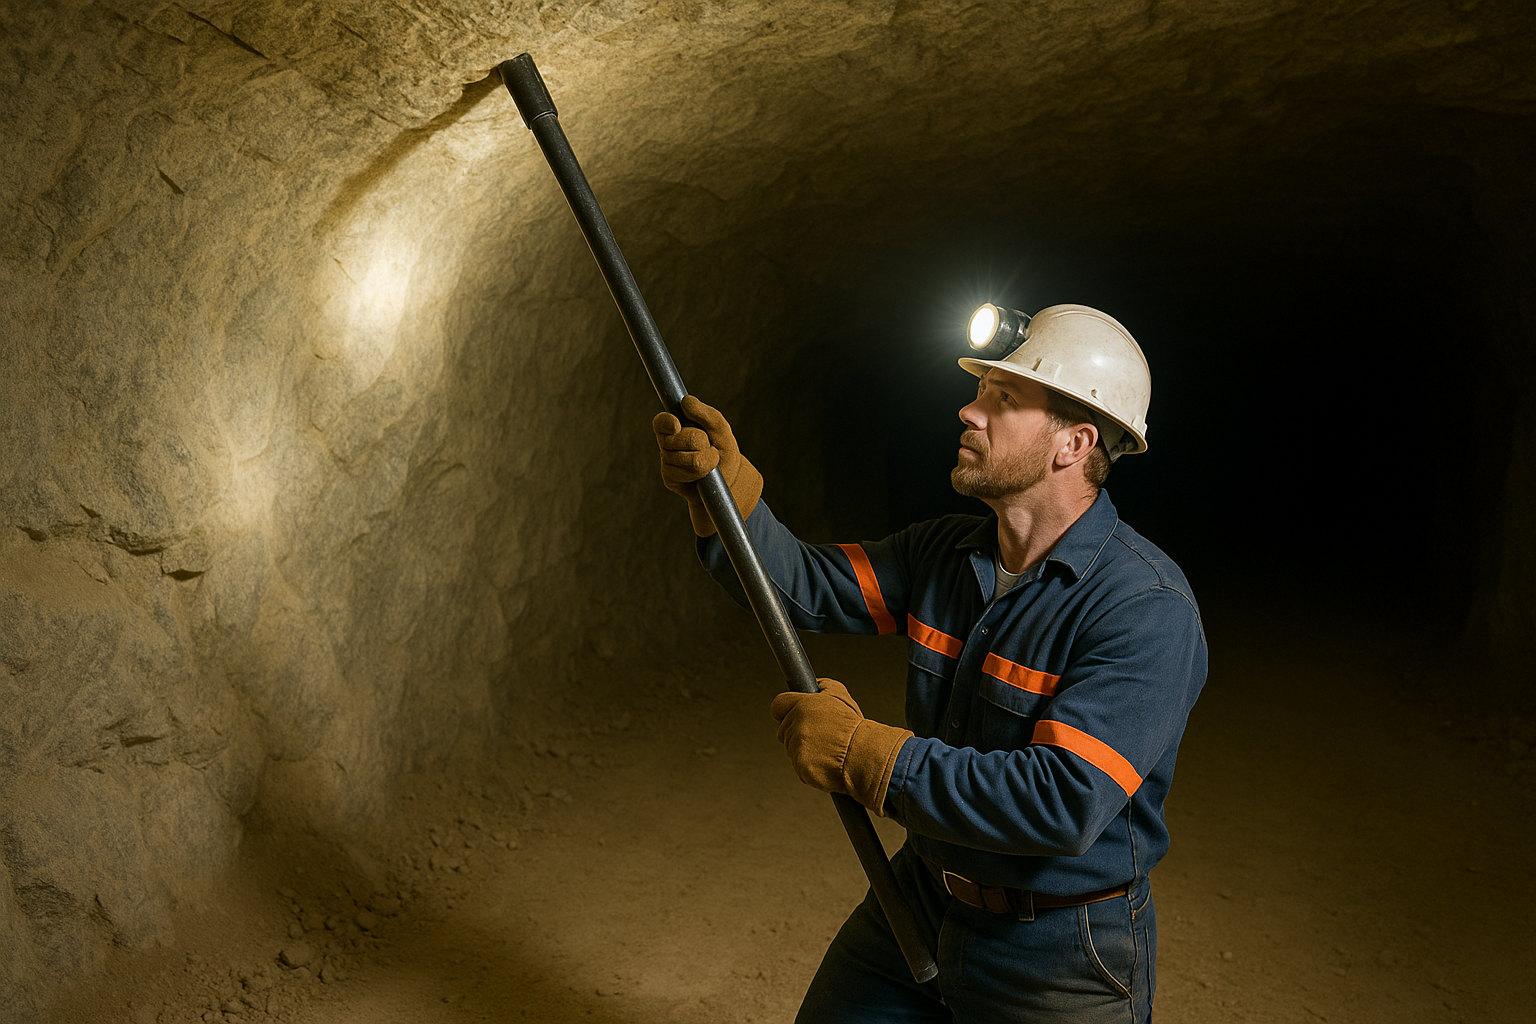
\includegraphics[width=\linewidth]{../assets/miner.png}
      \caption{AI generated image of a miner using a scaling bar}
      \label{fig:scaling_bar}
    \end{figure}
  \end{column}
\end{columns}

\end{frame}

%---------------------------------------------------------
\begin{frame}{Project Overview}
\begin{columns}[T,onlytextwidth]
  % Reduce font size for text
  \begin{column}{0.6\textwidth}
    \scriptsize % or \footnotesize if you want slightly larger
    \begin{itemize}
      \item Evaluating whether an impact sounds tight or drummy is a subjective process that requires training and experience.
      \item Some conditions can be difficult even for experienced miners, such as intersecting rooms and high roofs.
      \item The project aims to develop a method of automatically classifying mine roof impacts, removing the subjective human factor.
      \item This is achieved by recording the sound of impacts and using machine learning to classify them as either ``Tight'' or ``Drummy''.
      \item Project phases:
        \begin{itemize}
          \scriptsize
          \item Phase 1: Data collection and initial classification using a simple ML model.
          \item Phase 2: Improved classification using a more complex model and additional data.
        \end{itemize}
    \end{itemize}
  \end{column}

  % Figures column
  \begin{column}{0.4\textwidth}
    \begin{figure}
      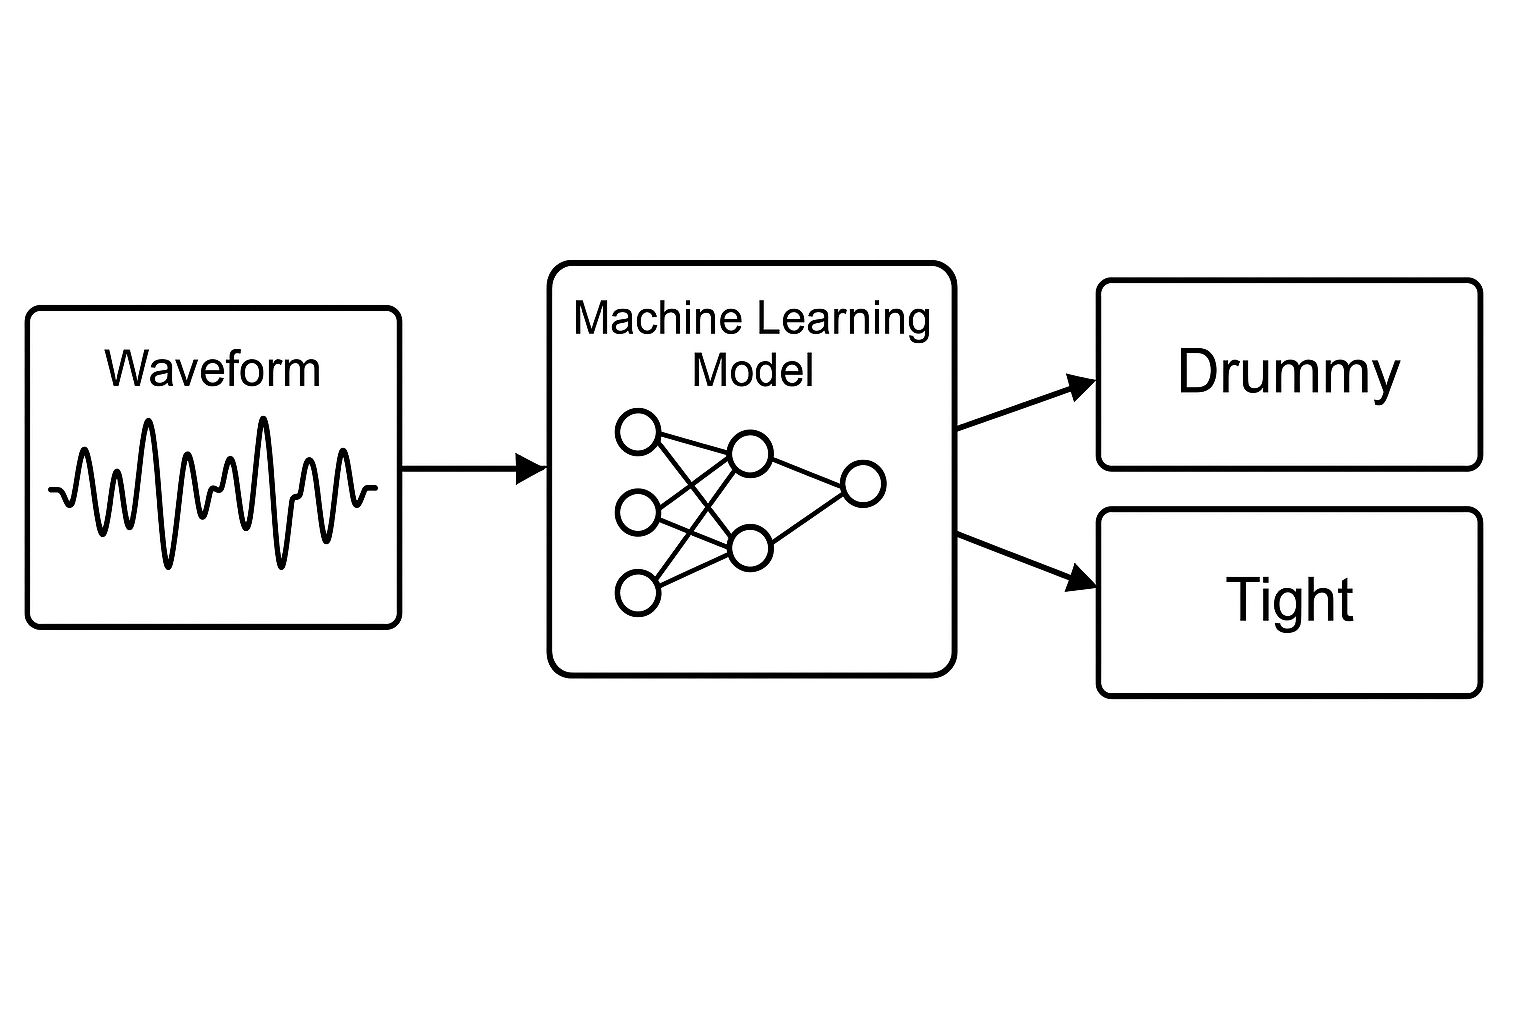
\includegraphics[width=40mm]{../assets/basic_pipeline.png}
      \caption{\scriptsize Classification Pipeline}
    \end{figure}
  \end{column}
  
\end{columns}
\end{frame}

%---------------------------------------------------------
\begin{frame}{Phase 1}
\begin{columns}[T,onlytextwidth]
  \begin{column}{0.6\textwidth}
    \scriptsize
    \begin{itemize}
      \item Phase 1 involved collecting data mine sits using a studio microphone setup.
      \item The data was recorded in Nutrien and Mosaic Potash Mines.
      \item Phase 1 Data consists of \textbf{3,309 recordings} (\textbf{2,212 drummy} sounds and \textbf{1,097 tight sounds}).Recordings in this phase have a duration of \textbf{0.75 seconds} and \textbf{36000 samples per recording}.
      \item The dataset is not balanced, with number of drummy sounds twice that of tight sounds. This means whenever we receive a model accuracy of \textbf{66\%} or less it is not better than random guessing.
    \end{itemize}
  \end{column}

  \begin{column}{0.4\textwidth}
    \begin{figure}
      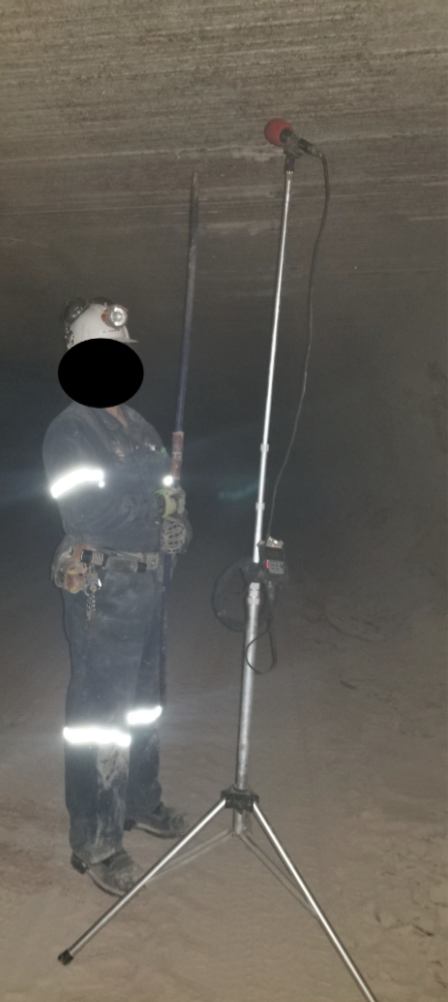
\includegraphics[width=25mm]{../assets/miner_micro.png}
      \caption{\scriptsize Phase 1 Microphone setup for recording impact sound}
    \end{figure}
  \end{column}
\end{columns}
\end{frame}

\begin{frame}{Phase 1 Data - Waveform Visualization}
    \begin{figure}
      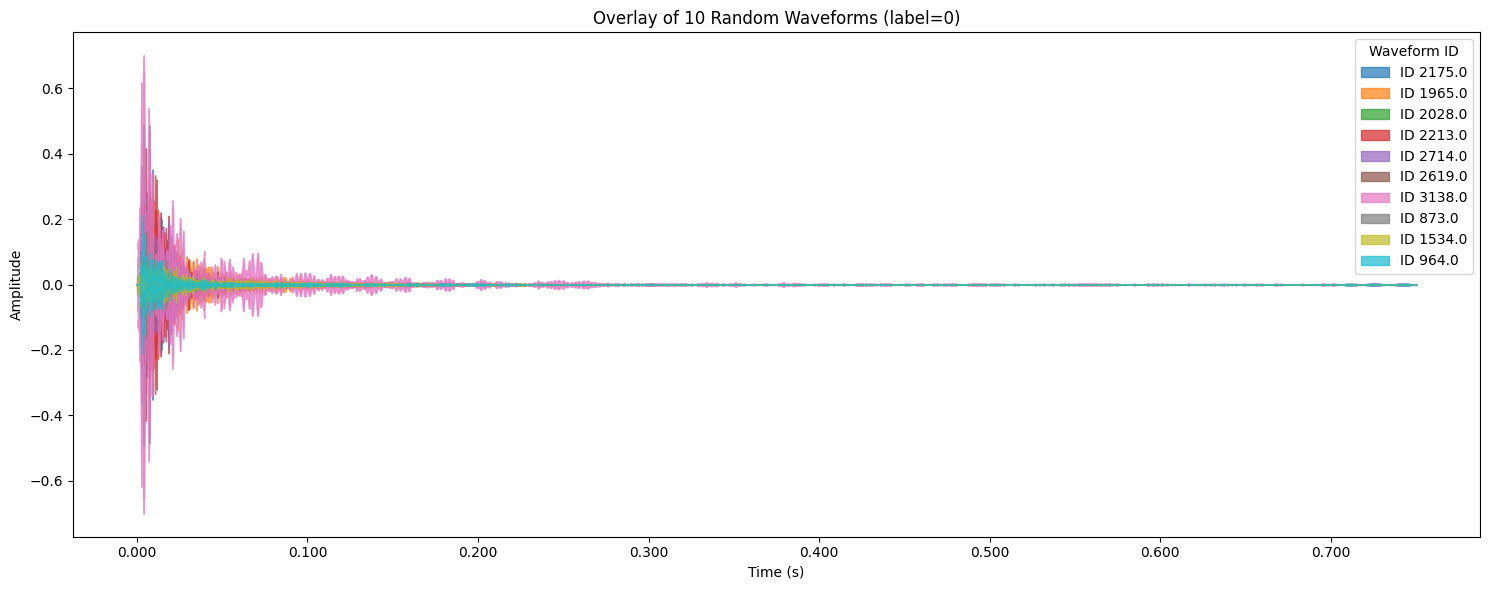
\includegraphics[width=0.6\textwidth]{../assets/final_report_assets/phase1_waveform_overlay_0.png}
      \caption{\scriptsize Waveform Overlay of Phase 1 Recordings Label 0(Drummy)}
      \label{fig:phase1_waveform_overlay_0}
    \end{figure}
    \begin{figure}
      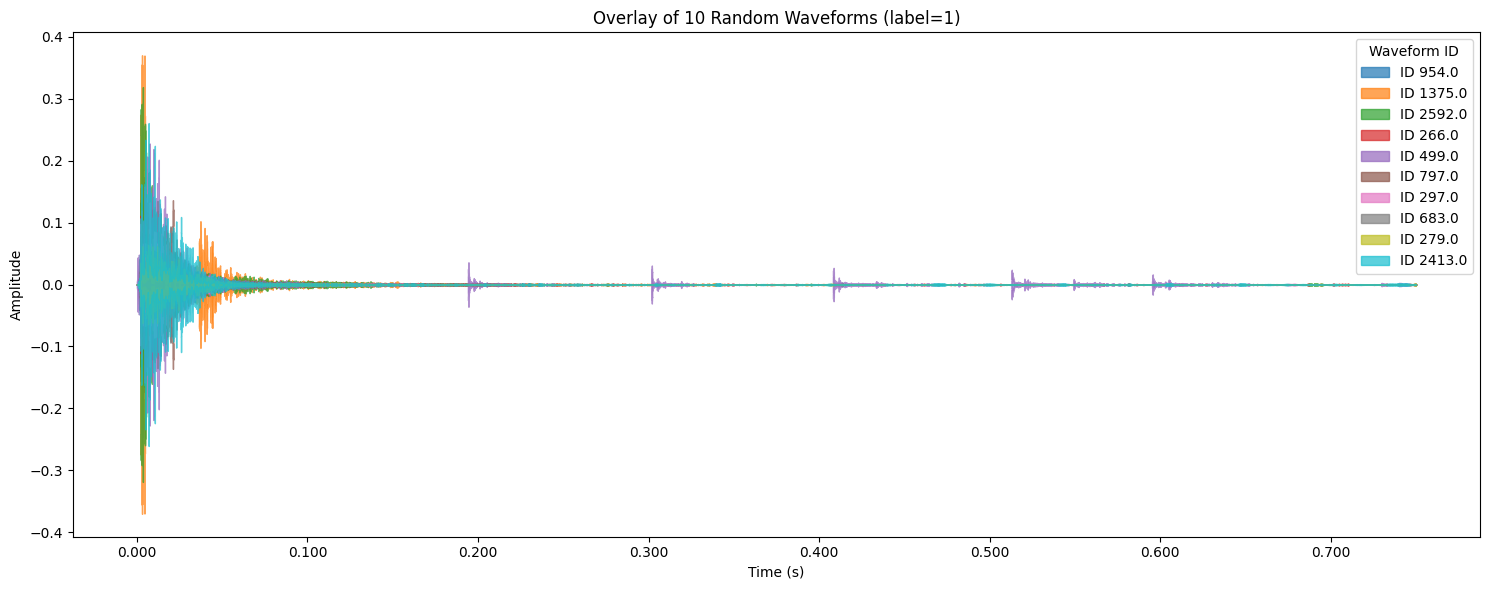
\includegraphics[width=0.6\textwidth]{../assets/final_report_assets/phase1_waveform_overlay_1.png}
      \caption{\scriptsize Waveform Overlay of Phase 1 Recordings Label 1(Tight)}
      \label{fig:phase1_waveform_overlay_1}
    \end{figure}

\end{frame}

%---------------------------------------------------------
\begin{frame}{Phase 2 }
\begin{columns}[onlytextwidth] % <-- remove [T]
  \begin{column}{0.6\textwidth}
    \scriptsize
    \begin{itemize}
      \item Phase 2 involved collecting data from mine sites using a custom device mounted on the scaling bar.
      \item Device Functionality:
        \begin{itemize}
          \scriptsize
          \item Detecting an impact 
          \item Recording the impact audio
          \item Allowing the user to label an impact as “drummy” or “tight” (optional)
          \item Transmitting the recording via Bluetooth to the app
          \item Receiving classifier results from the app
          \item Displaying the classifier results via the RGB LED 
        \end{itemize}
      \item Phase 2 data consists of \textbf{9,923 recordings} (from which \textbf{1,483} were \textbf{NaN-corrupted}, making it 8,440; plus some mis-hits to clean).
      \item \textbf{Upon removing mis-hits} with manual identification of waveforms, the final number of recordings is \textbf{8229}.
    \end{itemize}
  \end{column}

  \begin{column}[c]{0.4\textwidth} % <-- vertically center this column
    \begin{figure}
      \centering
      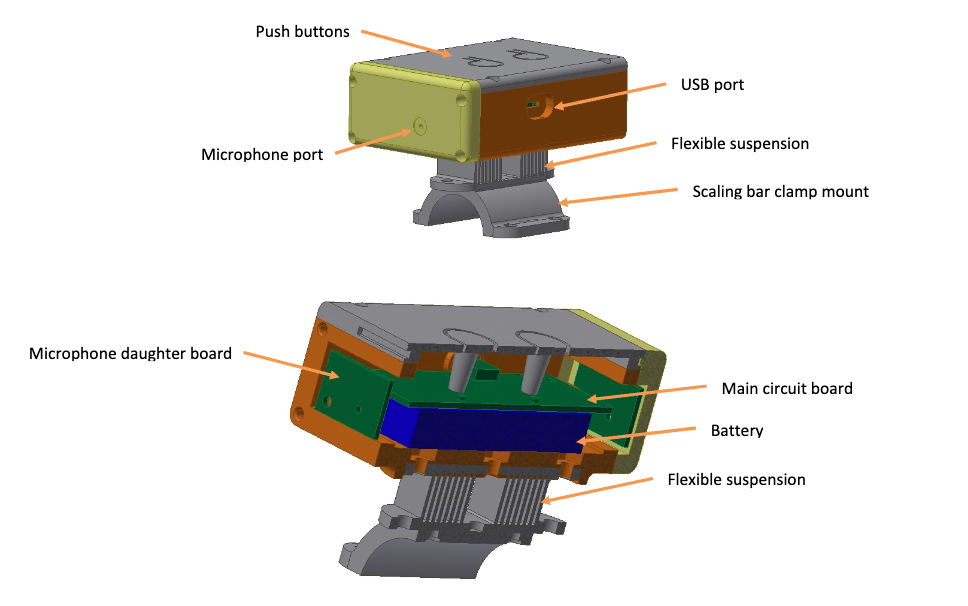
\includegraphics[width=50mm]{../assets/phase2_device.png}
      \caption{\scriptsize Phase 2 custom device mounted on a scaling bar}
    \end{figure}
  \end{column}
\end{columns}
\end{frame}
%---------------------------------------------------------
\begin{frame}{Phase 2 Data- Waveform Visualization}
    \begin{figure}
      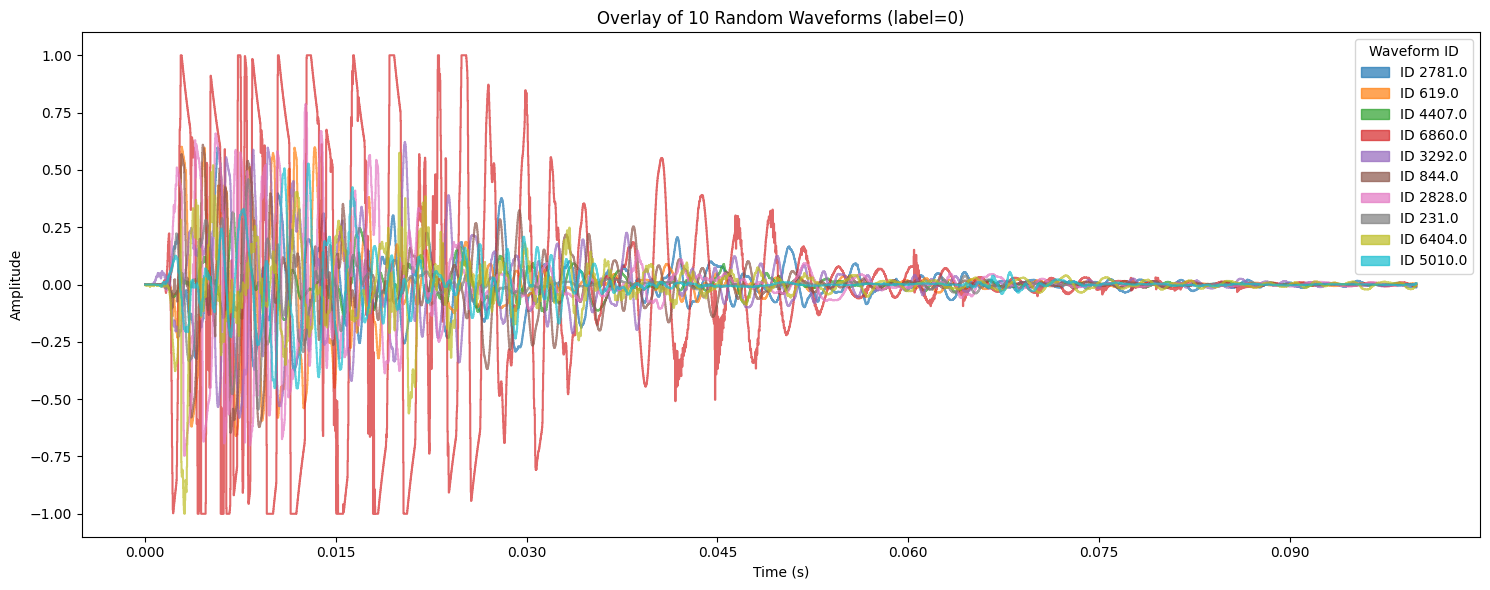
\includegraphics[width=0.6\textwidth]{../assets/final_report_assets/phase2_waveform_overlay_0.png}
      \caption{\scriptsize Waveform Overlay of Phase 2 Recordings Label 0(Drummy)}
      \label{fig:phase2_waveform_overlay_0}
    \end{figure}
    \begin{figure}
      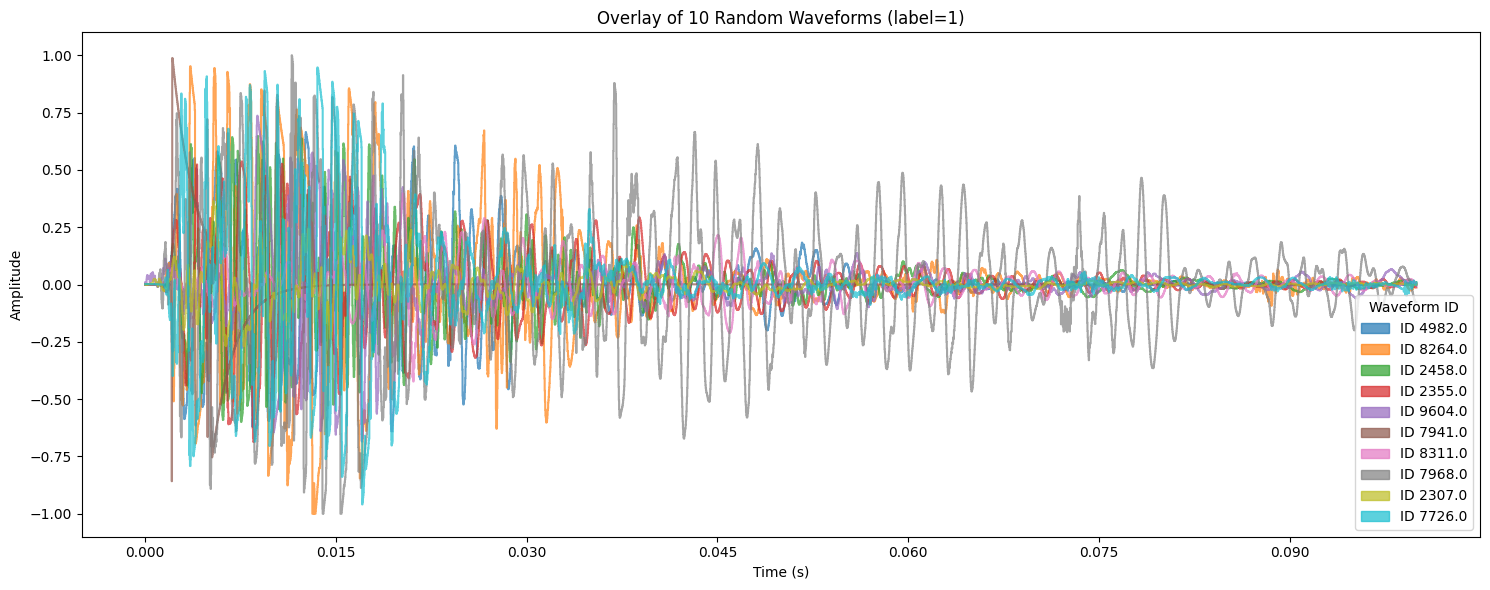
\includegraphics[width=0.6\textwidth]{../assets/final_report_assets/phase2_waveform_overlay_1.png}
      \caption{\scriptsize Waveform Overlay of Phase 2 Recordings Label 1(Tight)}
      \label{fig:phase2_waveform_overlay_1}
    \end{figure}
\end{frame}
%---------------------------------------------------------
\begin{frame}{Phase 2 Data- Mishits}
  \begin{figure}
    \centering

    % --- Top row ---
    \begin{minipage}{0.4\textwidth}
      \centering
      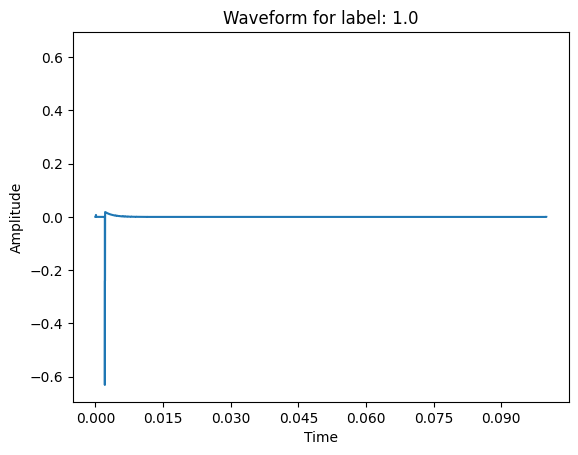
\includegraphics[width=35mm]{../assets/phase2_mishit_1.png}
      \caption{\scriptsize Phase 2 Mishit Recordings Label 1 (Tight)}
      \label{fig:phase2_mishit_0}
    \end{minipage}
    \hfill
    \begin{minipage}{0.4\textwidth}
      \centering
      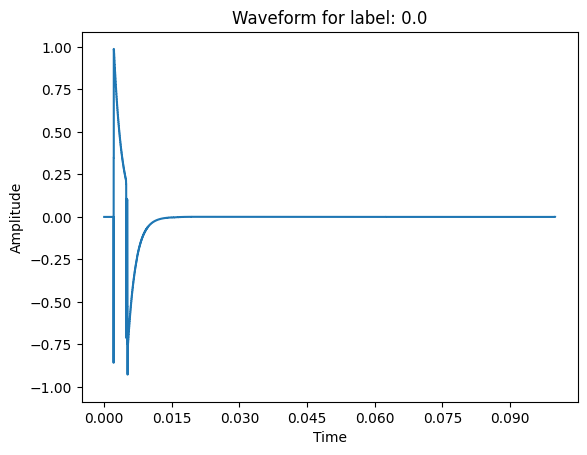
\includegraphics[width=35mm]{../assets/phase2_mishit_0.png}
      \caption{\scriptsize Phase 2 Mishit Recordings Label 0 (Drummy)}
      \label{fig:phase2_mishit_1}
    \end{minipage}


    % --- Bottom row ---
    \begin{minipage}{0.4\textwidth}
      \centering
      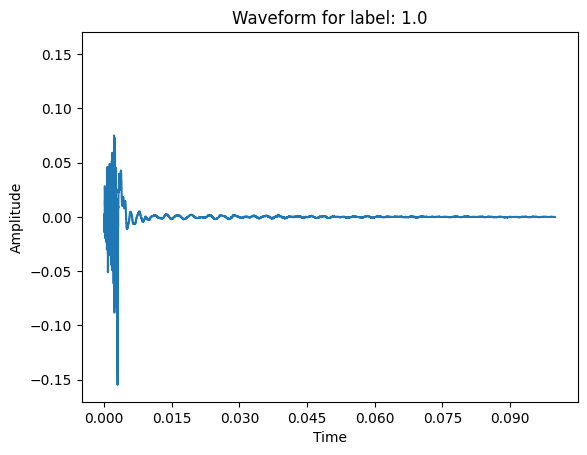
\includegraphics[width=35mm]{../assets/phase2_mishit_1_1.png}
      \caption{\scriptsize Phase 2 Mishit Recordings Label 1 (Tight)}
      \label{fig:phase2_mishit_1_1}
    \end{minipage}
    \hfill
    \begin{minipage}{0.4\textwidth}
      \centering
      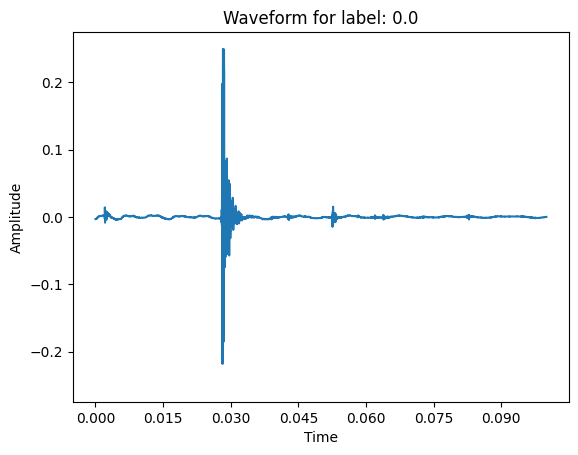
\includegraphics[width=35mm]{../assets/phase2_mishit_0_1.png}
      \caption{\scriptsize Phase 2 Mishit Recordings Label 0 (Drummy)}
      \label{fig:phase2_mishit_0_1}
    \end{minipage}

  \end{figure}
\end{frame}

\begin{frame}{PCA and classification}

    \begin{itemize}
      \item PCA was applied for dimensionality reduction and feature extraction, and explained variance was used to score features.
      \item SVM and other linear classifiers were used in Phase 1 of the project that could only yield around 80\% accuracy.   
      \item Comparison was done between using SVM and MLP as classifiers and found that MLP performed better than SVM almost always.
      \item 80\% Train Set and 20\% Test Set was used for training and testing the model for both dataset.
    \end{itemize}

\end{frame}
\begin{frame}{PCA on Phase 1 Data}
    \begin{figure}
      \centering
      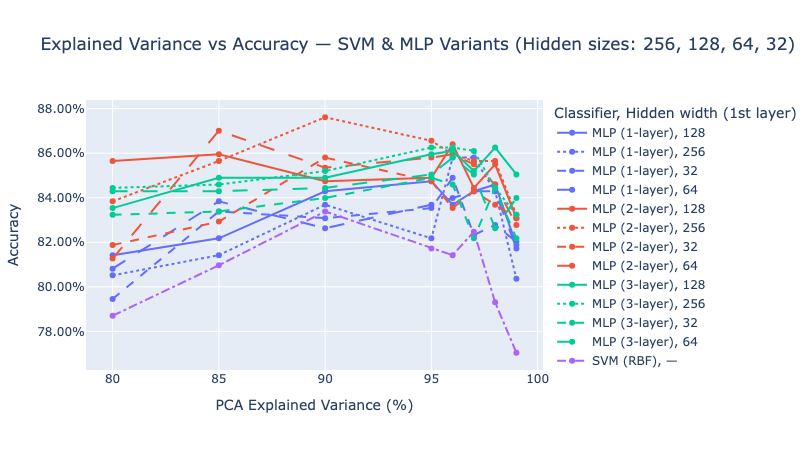
\includegraphics[width=1\textwidth]{../assets/final_report_assets/phase1_pca_explained_variance.png}
      \caption{\scriptsize Phase 1 PCA Explained Variance vs Accuracy (Over Multiple Models)}
      \label{fig:phase1_pca_explained_variance}
    \end{figure}
\end{frame}

\begin{frame}{PCA on Phase 1 Data (Best Model)}

\begin{minipage}{0.3\textwidth}
  \footnotesize
  \begin{table}
    \caption{\scriptsize 90\% var., MLP 256 hidden (Layer 1) - 128 hidden (Layer 2), dropout 0.2}
    \vspace{0.2em}
    \centering
    \begin{tabular}{@{}lccc r@{}}
      \toprule
      {} & precision & recall & f1-score & support \\
      \midrule
      drummy (0)   & 0.88 & 0.91 & 0.89 & 443 \\
      tight (1)    & 0.80 & 0.74 & 0.77 & 219 \\
      \midrule
      accuracy     & \multicolumn{3}{c}{0.85} & 662 \\
      macro avg    & 0.84 & 0.83 & 0.83 & 662 \\
      weighted avg & 0.85 & 0.85 & 0.85 & 662 \\
      \bottomrule
    \end{tabular}
    \vspace{0.3em}
    {\scriptsize [RETRAIN] Accuracy (report{=}True): 0.8535}
  \end{table}
\end{minipage}%
\hfill
\begin{minipage}{0.3\textwidth}
  \centering
  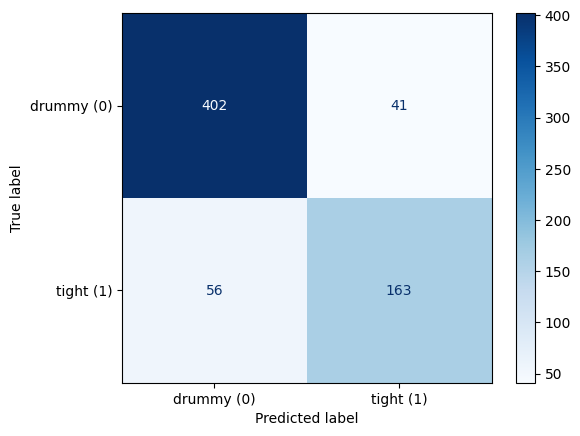
\includegraphics[width=30mm]{../assets/final_report_assets/phase1_pca_best_confusion.png}
  \caption{\scriptsize Phase 1 PCA Best Confusion Matrix}
  \label{fig:phase1_pca_best_confusion}
\end{minipage}

\end{frame}

\begin{frame}{PCA on Phase 1 Data (Best Model Architecture)}
    \begin{figure}
      \centering
      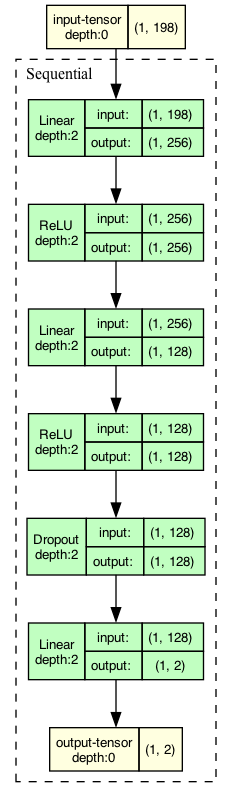
\includegraphics[width=0.18\textwidth]{../assets/final_report_assets/best_model_mlp2_ev90_h256_P1_RETRAIN.png}
      \caption{\scriptsize Phase 1 PCA Best Model Architecture}
      \label{fig:phase1_pca_best_model_architecture}
    \end{figure}
\end{frame}


\begin{frame}{PCA on Phase 2 Data}
    \begin{figure}
      \centering
      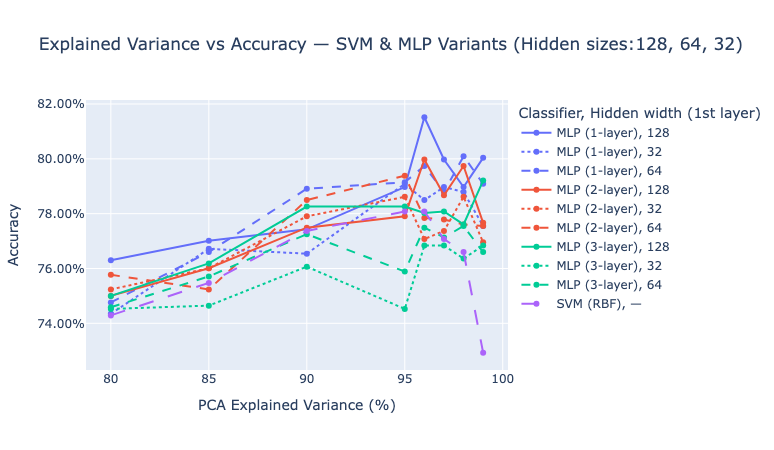
\includegraphics[width=1\textwidth]{../assets/final_report_assets/phase2_pca_explained_variance.png}
      \caption{\scriptsize Phase 2 PCA Explained Variance vs Accuracy (Over Multiple Models)}
      \label{fig:phase2_pca_explained_variance}
    \end{figure}
\end{frame}
\begin{frame}{PCA on Phase 2 Data (Best Model)}
\begin{minipage}{0.3\textwidth}
  \footnotesize
  \begin{table}
    \caption{\scriptsize 96\% var., MLP 128 hidden (Layer 1), dropout 0.2}
    \vspace{0.2em}
    \centering
    \begin{tabular}{@{}lccc r@{}}
      \toprule
      {} & precision & recall & f1-score & support \\
      \midrule
      drummy (0)   & 0.78 & 0.86 & 0.82 & 926 \\
      tight (1)    & 0.81 & 0.71 & 0.75 & 762 \\
      \midrule
      accuracy     & \multicolumn{3}{c}{0.79} & 1688 \\
      macro avg    & 0.80 & 0.79 & 0.79 & 1688 \\
      weighted avg & 0.79 & 0.79 & 0.79 & 1688 \\
      \bottomrule
    \end{tabular}
    \vspace{0.3em}
    {\scriptsize [RETRAIN] Accuracy (report{=}True): 0.7927}
  \end{table}
\end{minipage}%
\hfill
\begin{minipage}{0.3\textwidth}
  \centering
  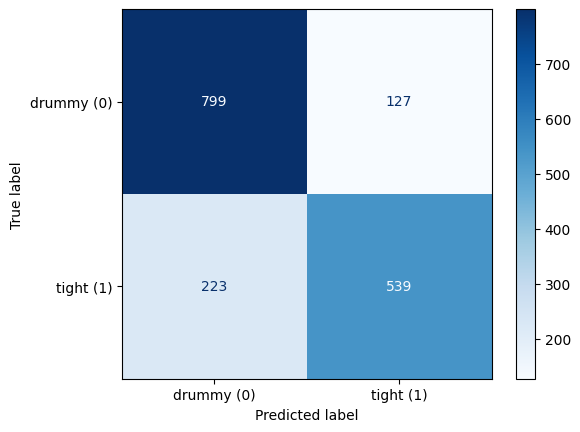
\includegraphics[width=30mm]{../assets/final_report_assets/phase2_pca_best_confusion.png}
  \caption{\scriptsize Phase 2 PCA Best Confusion Matrix}
  \label{fig:phase2_pca_best_confusion}
\end{minipage}
\end{frame}
\begin{frame}{PCA on Phase 2 Data (Best Model Architecture)}
    \begin{figure}
      \centering
      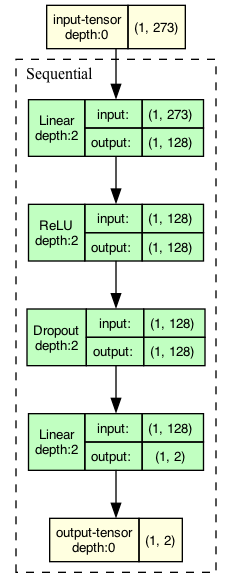
\includegraphics[width=0.18\textwidth]{../assets/final_report_assets/best_model_mlp1_ev96_h128_P2_RETRAIN.png}
      \caption{\scriptsize Phase 2 PCA Best Model Architecture}
      \label{fig:phase2_pca_best_model_architecture}
    \end{figure}
  \end{frame}

\begin{frame}{Deep Learning Models and Generalization techniques}
  \scriptsize
  \begin{itemize}
    \item PCA is a powerful technique for dimensionality reduction and feature extraction, but it is not always the best choice for all datasets especially when we have temporal data.
    \item As seen with PCA and MLP, neural networks greatly outperform SVMs hence more complex models can be used to greatly improve accuracy.
    \item For Phase 1, an end-to-end ResNet model was developed.
    \item For Phase 2, an end-to-end ResNet model, MFCC + MLP and MFCC + ResNet models were developed.
    \item 90\% train set and 10\% test set was used for training and testing the model for both dataset.
    \item Generalization Techniques
    \scriptsize
    \begin{itemize}
      \scriptsize
      \item Tanh activations after every convolutional stage→consistent smoothing of feature maps.
      \item BatchNorm1d applied to output of the first ResidualBlock→stabilized feature statistics.
      \item Dropout(0.6) in the classifier head→stronger regularization.
      \item Label smoothing ε=0.1 carried over for consistent training behavior.
    \end{itemize}
  \end{itemize}
\end{frame}

\begin{frame}{Phase 1 ResNet Model (Architecture)}
    \begin{figure}
      \centering
      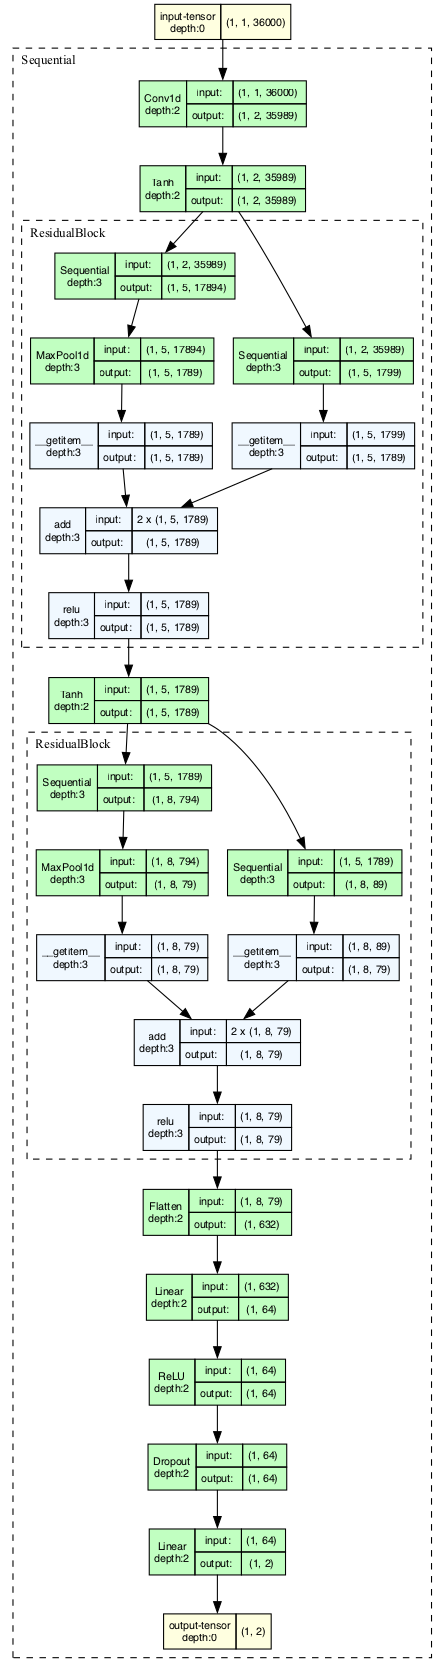
\includegraphics[width=0.15\textwidth]{../assets/final_report_assets/conv_p1_model_arch.png}
      \caption{\scriptsize Phase 1 CNN Model Architecture}
      \label{fig:phase1_cnn_model_architecture}
    \end{figure}

\end{frame}

% Preamble (if not already present)
% \usepackage{booktabs}
% \usepackage{caption}

\begin{frame}{Phase 1 ResNet Model (Performance)}
\begin{minipage}{0.3\textwidth}
  \footnotesize
  \begin{table}
    \caption{Epochs=20, Batch Size=32,  LR=0.001, Dropout=0.6}
    \vspace{0.2em}
    \centering
    \begin{tabular}{@{}lccc r@{}}
      \toprule
      {} & precision & recall & f1-score & support \\
      \midrule
      drummy (0)   & 1.00 & 0.98 & 0.99 & 221 \\
      tight (1)    & 0.96 & 0.99 & 0.97 &  88 \\
      \midrule
      accuracy     & \multicolumn{3}{c}{0.98} & 309 \\
      macro avg    & 0.98 & 0.99 & 0.98 & 309 \\
      weighted avg & 0.98 & 0.98 & 0.98 & 309 \\
      \bottomrule
    \end{tabular}
  \end{table}
\end{minipage}%
\hfill
\begin{minipage}{0.3\textwidth}
  \centering
  \begin{figure}
  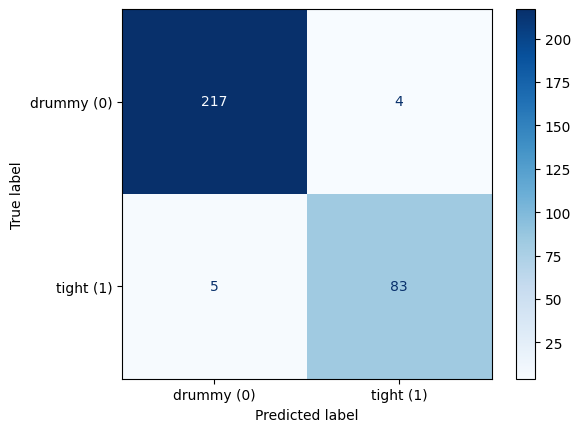
\includegraphics[width=30mm]{../assets/new_arch_conv_p1.png}
  \caption{\scriptsize Phase 1 ResNet Confusion Matrix}
  \label{fig:phase1_resnet_confusion}
  \end{figure}
\end{minipage}
\end{frame}

\begin{frame}{Phase 2 ResNet Model (Architecture)}
    \begin{figure}
      \centering
      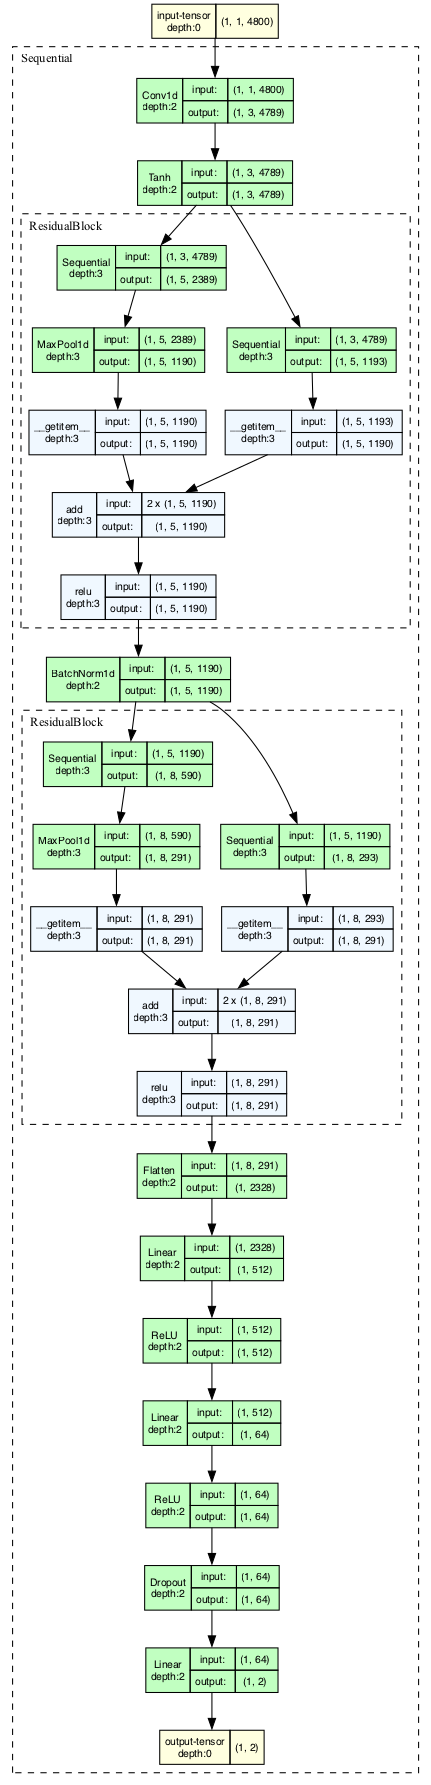
\includegraphics[width=0.15\textwidth]{../assets/final_report_assets/conv_p2_model_arch.png}
      \caption{\scriptsize Phase 2 CNN Model Architecture}
      \label{fig:phase2_cnn_model_architecture}
    \end{figure}
  
\end{frame}

\begin{frame}{Phase 2 ResNet Model (Performance)}
\begin{minipage}{0.3\textwidth}
  \footnotesize
  \begin{table}
    \caption{Epochs=20, Batch Size=90,  LR=0.001, Dropout=0.6, Weight\_Decay=0.001}
    \vspace{0.2em}
    \centering
    \begin{tabular}{@{}lccc r@{}}
      \toprule
      {} & precision & recall & f1-score & support \\
      \midrule
      drummy (0)   & 0.87 & 0.92 & 0.90 & 466 \\
      tight (1)    & 0.89 & 0.83 & 0.86 & 363 \\
      \midrule
      accuracy     & \multicolumn{3}{c}{0.88} & 829 \\
      macro avg    & 0.88 & 0.88 & 0.88 & 829 \\
      weighted avg & 0.88 & 0.88 & 0.88 & 829 \\
      \bottomrule
    \end{tabular}
  \end{table}
\end{minipage}%
\hfill
\begin{minipage}{0.3\textwidth}
  \centering
  \begin{figure}
    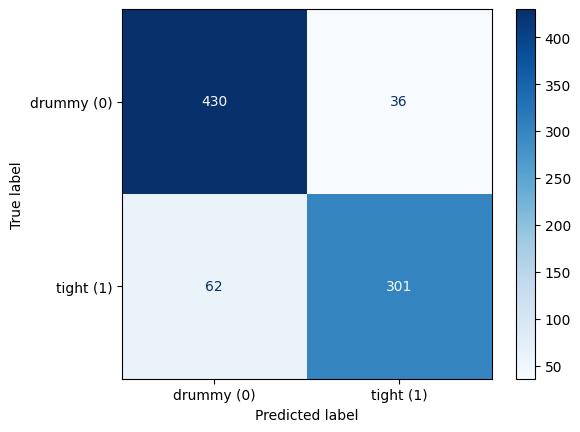
\includegraphics[width=30mm]{../assets/phase2_resnet_confusion.png} % <-- replace with your actual Phase 2 confusion matrix path
    \caption{\scriptsize Phase 2 ResNet Confusion Matrix}
    \label{fig:phase2_resnet_confusion}
  \end{figure}
\end{minipage}
\end{frame}

\begin{frame}{Phase 2 MFCC + MLP Model (Architecture)}
    \begin{figure}
      \centering
      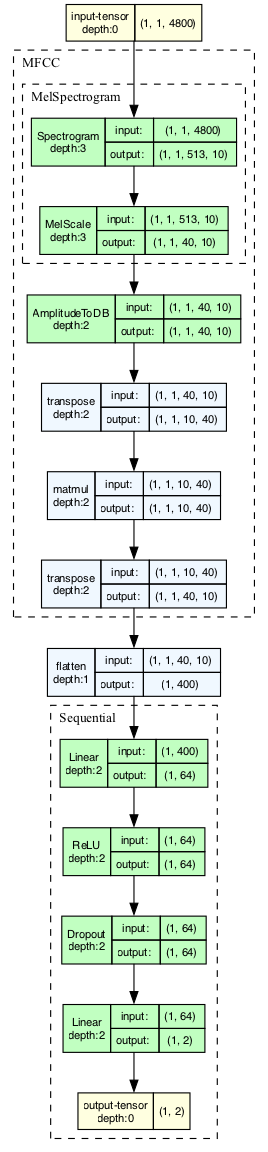
\includegraphics[width=0.15\textwidth]{../assets/final_report_assets/mfcc_p2_model_arch.png}
      \caption{\scriptsize Phase 2 MFCC + MLP Model (Architecture)}
      \label{fig:phase2_MFCC_model_architecture}
    \end{figure}
\end{frame}

\begin{frame}{Phase 2 MFCC + MLP Model (Performance)}
\begin{minipage}{0.3\textwidth}
  \footnotesize
  \begin{table}
    \caption{\scriptsize Input: torch.Size([1, 4800]), MFCC + MLP, n\_mfcc=40, n\_fft=1024, hop\_length=512, n\_mels=40}
    \vspace{0.2em}
    \centering
    \begin{tabular}{@{}lccc r@{}}
      \toprule
      {} & precision & recall & f1-score & support \\
      \midrule
      drummy (0)   & 0.91 & 0.90 & 0.91 & 466 \\
      tight (1)    & 0.88 & 0.89 & 0.88 & 363 \\
      \midrule
      accuracy     & \multicolumn{3}{c}{0.90} & 829 \\
      macro avg    & 0.89 & 0.90 & 0.89 & 829 \\
      weighted avg & 0.90 & 0.90 & 0.90 & 829 \\
      \bottomrule
    \end{tabular}
  \end{table}
\end{minipage}%
\hfill
\begin{minipage}{0.3\textwidth}
  \centering
  \begin{figure}
    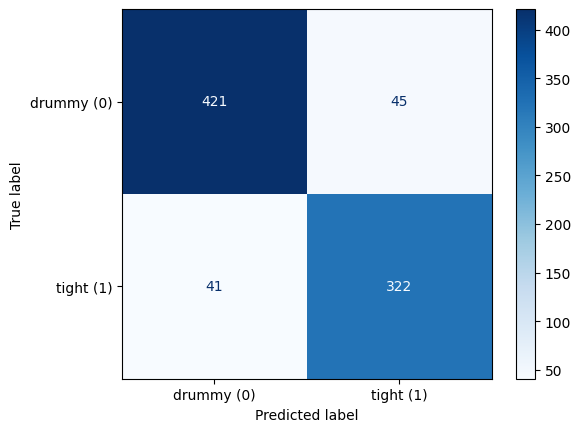
\includegraphics[width=30mm]{../assets/phase2_mfcc_mlp_confusion.png} % <-- replace with actual confusion matrix image
    \caption{\scriptsize Phase 2 MFCC + MLP Confusion Matrix}
    \label{fig:phase2_mfcc_mlp_confusion}
  \end{figure}
\end{minipage}
\end{frame}


\begin{frame}{Phase 2 MFCC + ResNet Model (Architecture)}
    \begin{figure}
      \centering
      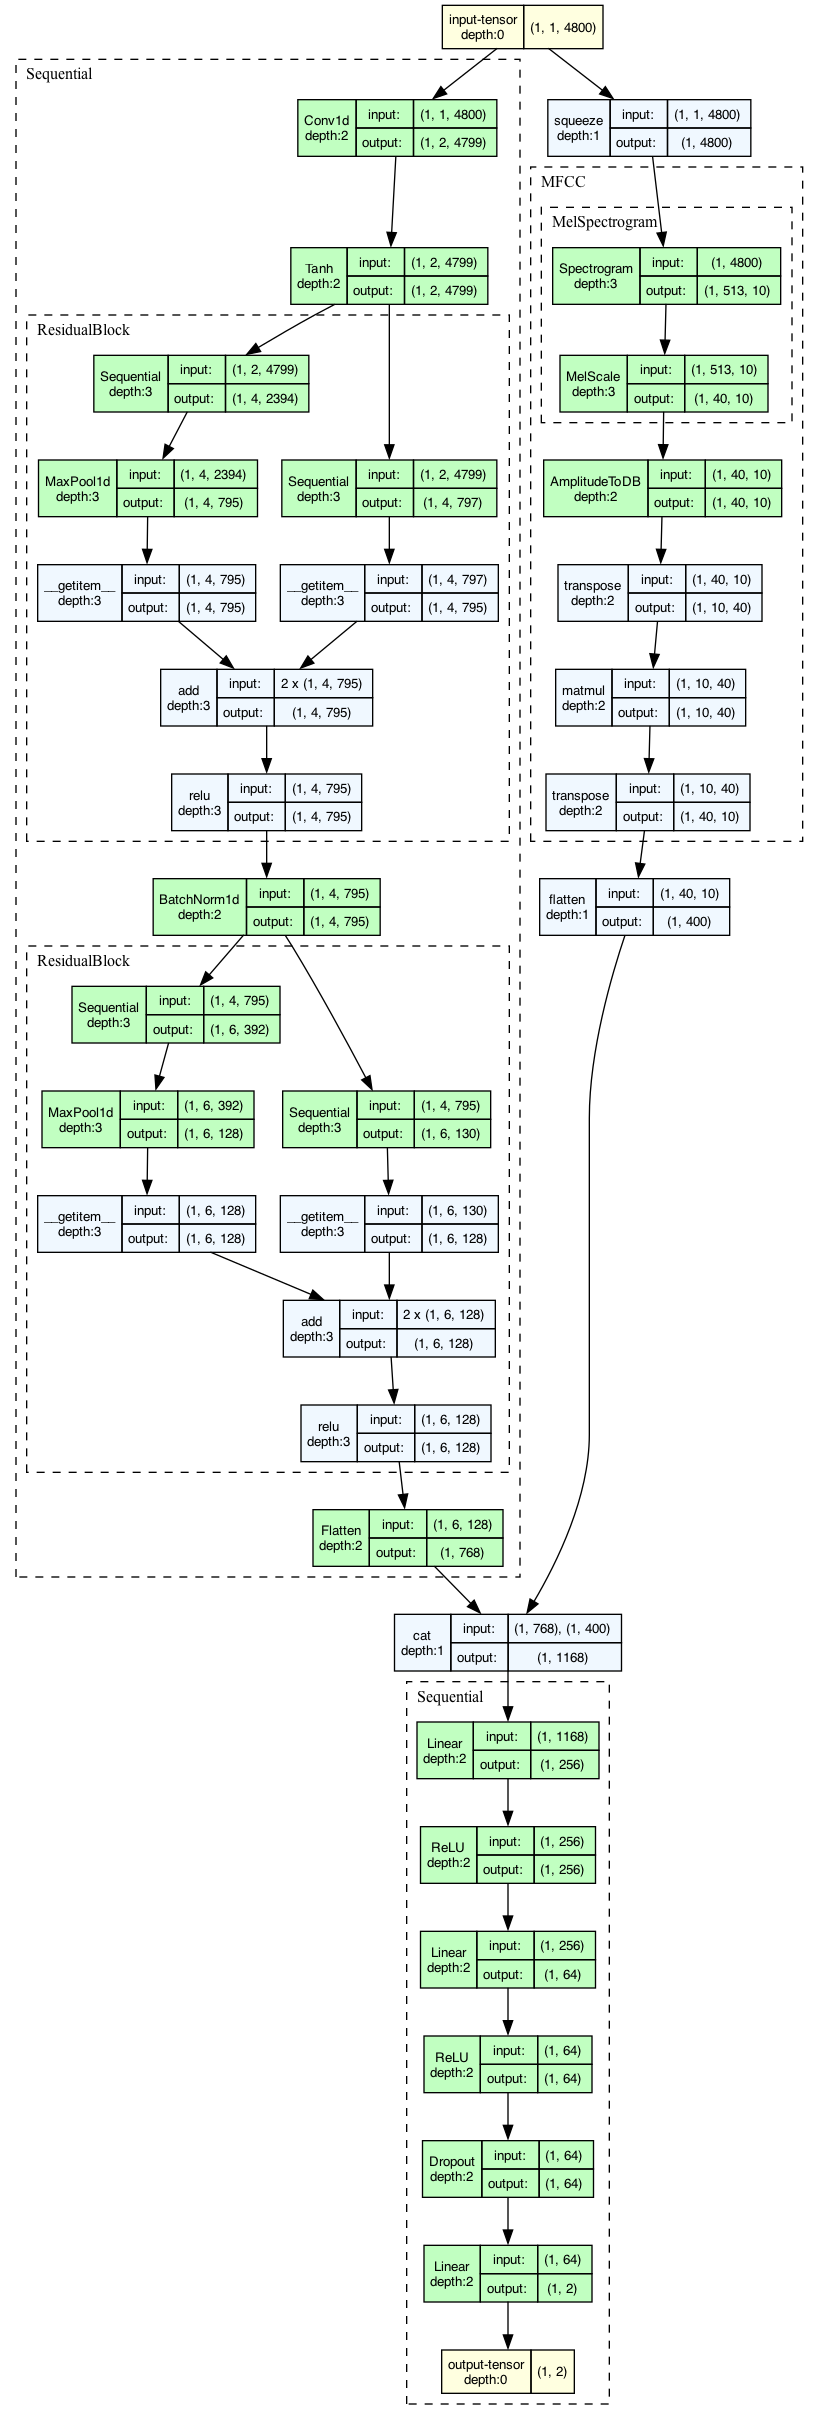
\includegraphics[width=0.15\textwidth]{../assets/final_report_assets/mfcc_resnet_p2_model_arch.png}
      \caption{\scriptsize Phase 2 MFCC + ResNet Model (Architecture)}
      \label{fig:phase2_MFCC_resnet_model_architecture}
    \end{figure}
\end{frame}
\begin{frame}{Phase 2 MFCC + ResNet Model (Performance)}
\begin{minipage}{0.3\textwidth}
  \footnotesize
  \begin{table}
    \caption{Input: MFCC, ResNet Backbone}
    \vspace{0.2em}
    \centering
    \begin{tabular}{@{}lccc r@{}}
      \toprule
      {} & precision & recall & f1-score & support \\
      \midrule
      drummy (0)   & 0.94 & 0.93 & 0.93 & 466 \\
      tight (1)    & 0.91 & 0.92 & 0.92 & 363 \\
      \midrule
      accuracy     & \multicolumn{3}{c}{0.93} & 829 \\
      macro avg    & 0.92 & 0.93 & 0.93 & 829 \\
      weighted avg & 0.93 & 0.93 & 0.93 & 829 \\
      \bottomrule
    \end{tabular}
  \end{table}
\end{minipage}%
\hfill
\begin{minipage}{0.3\textwidth}
  \centering
  \begin{figure}
    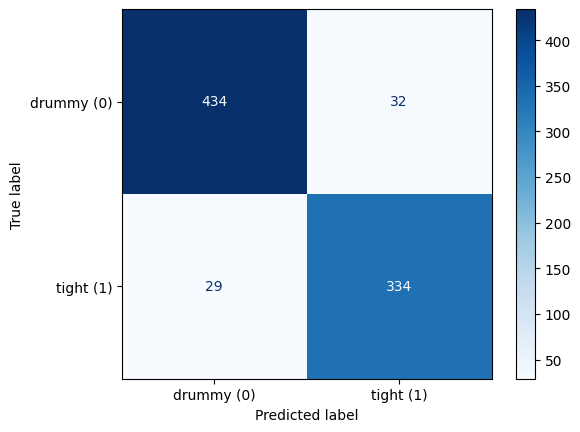
\includegraphics[width=30mm]{../assets/phase2_mfcc_resnet_confusion.png} % <-- replace with actual confusion matrix image
    \caption{\scriptsize Phase 2 MFCC + ResNet Confusion Matrix}
    \label{fig:phase2_mfcc_resnet_confusion}
  \end{figure}
\end{minipage}
\end{frame}

\begin{frame}{Model Discussion}
  \scriptsize
\begin{itemize}
    \item In Phase 1, the classification task has been pushed to its limits — the end-to-end \textbf{ResNet} model achieved \textbf{98.38\% accuracy}, outperforming even MFCC-based approaches.
    \item Across Phase 2 experiments, the \textbf{MFCC + ResNet} model achieved the highest \textbf{F1-score} overall, followed closely by the \textbf{MFCC + MLP} model.
    \item In terms of class-level performance:
        \begin{itemize}
          \scriptsize
            \item \textbf{MFCC + ResNet} showed more balanced \textbf{recall} across both “drummy” and “tight” classes, indicating better discrimination.
            \item \textbf{MFCC + MLP} also performed well but had slightly less balanced recall, suggesting a small bias towards one class.
        \end{itemize}
    \item Incorporating \textbf{label smoothing} led to an accuracy increase of approximately \textbf{+2\%}, likely due to reducing overconfidence and improving generalization.
    \item Adding a \textbf{tanh activation} after convolution layers contributed another \textbf{+2\%} accuracy gain.
        \begin{itemize}
          \scriptsize
            \item \textbf{Intuition:} \texttt{tanh} preserves negative values, which may store important information about waveform amplitudes — especially for oscillatory signals where polarity matters.
        \end{itemize}
\end{itemize}
\end{frame}

\begin{frame}{Future Work}
\begin{itemize}

    \item Address the challenge of having two distinct datasets (Phase 1 and Phase 2) with different input dimensions:
        \begin{itemize}
            \scriptsize
            \item Phase 1 recordings: 0.75s duration, 36000 samples.
            \item Phase 2 recordings: 0.1s duration, 4800 samples.
        \end{itemize}
        \begin{itemize}
            \scriptsize
            \item Current approach involves resampling one dataset to match the other, which may lead to loss of information or introduce artifacts.
            \item A more elegant solution is needed to handle both datasets without resampling.
        \end{itemize}
    \item Develop a unified model architecture that can \textbf{process both dataset types} directly, without needing to resample the data to match a single fixed input dimension.
    \item Implement a more \textbf{robust preprocessing} pipeline:
        \begin{itemize}
            \scriptsize
            \item Here, \textbf{robust} means capable of automatically detecting and removing \textbf{mishits} or invalid recordings before feature extraction.
            \item This would involve statistical anomaly detection or learned filtering like similarity search with manually identified mishits to ensure only valid impacts are classified.
        \end{itemize}
    
\end{itemize}
\end{frame}


\begin{frame}{Conclusion}
\begin{itemize}
    \item Multiple architectures were evaluated for Phase 2 classification, with \textbf{MFCC + ResNet} emerging as the top performer in terms of both accuracy and balanced recall.
    \item Small architectural changes — such as \textbf{label smoothing} and \textbf{tanh after convolution layers} — provided measurable improvements of around \textbf{+2\% accuracy each}.
    \item Results indicate that incorporating feature diversity (MFCC + CNN) and preserving negative activations can enhance the ability to discriminate between “drummy” and “tight” impacts.
    \item Future work will aim to unify dataset handling and improve preprocessing to ensure consistently high-quality inputs.
\end{itemize}
\end{frame}

\end{document}